\documentclass[11pt]{article}
\usepackage[preprint]{acl}
\usepackage{times}
\usepackage{latexsym}
\usepackage[T1]{fontenc}
\usepackage[utf8]{inputenc}
\usepackage{microtype}
\usepackage{inconsolata}
\usepackage{graphicx}
\usepackage{booktabs}
\usepackage{amsmath}
\usepackage{amssymb}
\usepackage{multirow}
\usepackage{xcolor}

\newcommand{\ci}[2]{\,{\scriptsize[#1,\,#2]}}
\newcommand{\rw}[2]{read~#1\,/\,write~#2}
\newcommand{\nat}[1]{native~#1/#1}

\title{Read Deep, Write Shallow: How Looped Language Models Should Spend Their Depth}

\author{Yang Hu}

\begin{document}
\maketitle

\begin{abstract}
Looped (recurrent-depth) language models run the same number of loops when reading the prompt and when writing the
answer. A small depth-split connector---LoRA plus per-loop key--value maps on a
frozen model---lets the prompt be read with $p$ loops and the answer written with $d$ loops. On Ouro-2.6B, the full
$4\times4$ map shows a division of labour: \emph{depth spent reading the prompt buys understanding, while depth spent
writing the answer buys multi-step derivation.} At one writing loop, reading 4 loops instead of 1 adds 15.2 MMLU and 8.6
RULER-16K points, and the effect replicates on five more checkpoints. On SenseNova-Loop-9B, whose one-loop writer
collapses, merely reading a two-loop prompt state, without any training, cuts unanswered GSM8K problems from 97\% to
44\%. Writing shallow is where time is saved: a connector writing two loops comes within one point of the 4-loop
Ouro-2.6B-Thinking on GSM8K at $0.55\times$ its time per answer. Through a RoPE-commuting key scale, one prompt KV cache
serves every loop exactly; storing the answer once too more than doubles long-answer decode throughput. Reading deep hurts short-context retrieval and few-shot mathematics, consistent with linear probes: deeper
loops keep less of what was said and more of what comes next.
\end{abstract}

\section{Introduction}

Looped language models such as Ouro~\citep{ouro}, Huginn~\citep{huginn} and Mixture-of-Recursions~\citep{mor}, in the
line of Universal Transformers~\citep{ut}, obtain depth without parameters by running a shared block of layers several
times per token. The price is paid at inference: every generated token runs every loop, and a cache per loop multiplies
decode memory. Yet the two phases of inference are not alike. Prefill is parallel and paid once per request; decode is
sequential and paid per generated token. A looped model nevertheless spends the same depth on both.

Unequal depths have been used before. Continuous Depth Batching runs full-depth prefill and exits early during
decode~\citep{cdb}; OverFill pairs a large prefill model with a small decoder~\citep{overfill}; Fixed Points Part~II
varies prefill recurrences at a fixed decode depth~\citep{fixedpoints2}. What has not been measured is \emph{what each
depth buys}. The obstacle is practical: a model that writes with fewer loops than it read with must attend to prompt
keys and values produced by a deeper loop than its own, and naive sharing breaks exactly where it would be most useful.
In our experiments, a trained terminal-KV sharing baseline loses 17.5 GSM8K points at one writing loop
(\S\ref{sec:ablations}).

We train one small connector on frozen checkpoints that makes every (read, write) pair up to four usable, and use it to
map the depth-allocation space (Figure~\ref{fig:grid}). Our contributions:
\begin{itemize}
\setlength\itemsep{0.15em}
\item \textbf{Read-deep / write-shallow, measured.} A $4\times4$ read $\times$ write map on Ouro-2.6B shows that
reading depth moves knowledge and long-context understanding while writing depth moves multi-step derivation; the
read-depth effect replicates on five more checkpoints. Effects of adaptation and of reading depth are reported
separately.
\item \textbf{Shallow-writer wandering, and what deep reading does to it.} One-loop writers of reasoning models often fail
to answer (43\% of GSM8K answers hit the budget on Ouro-2.6B-Thinking; 97\% end without a final answer on
SenseNova-Loop-9B). With the writer fixed, reading
deeper makes it finish more often and answer more briefly, most on the hardest problems---without any training on
SenseNova. Its hesitation density per token does not change; it reaches an answer sooner.
\item \textbf{RoPE-commuting KV maps.} A per-frequency complex scale on keys commutes with rotary embeddings~\citep{rope},
so it can be folded into the query; with a post-attention value map, one stored prompt cache serves every decode loop
exactly. Trained in the inference-time (self-live) view, one shared answer bank matches per-loop answer banks at two to three
writing loops and, on long answers, more than doubles decode throughput at four (at a 2.6-point GSM8K cost).
\item \textbf{Shallow KV keeps what was said, deep KV keeps what comes next.} Our failure cases (verbatim retrieval,
few-shot mathematics) and the opposite first-loop / last-loop sharing choices of prior work are consistent with one
pattern, which linear probes of the cache reproduce and a prompting control supports: on MATH-500, reading deep costs 9.8
points with four exemplars and gains 7.0 without them.
\end{itemize}

\begin{figure*}[t]
\centering
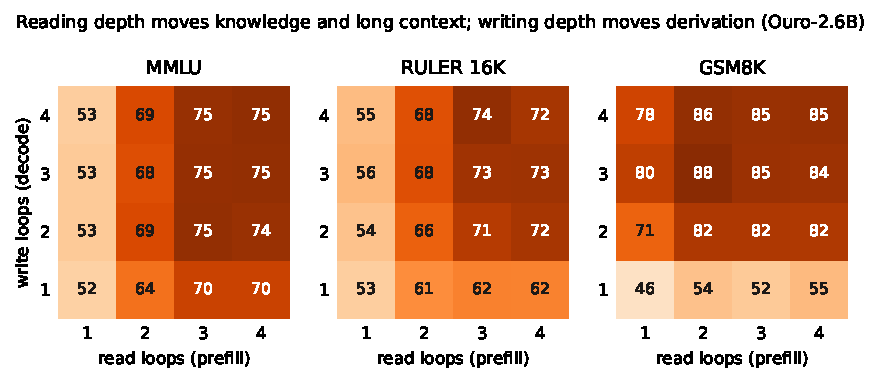
\includegraphics[width=0.92\textwidth]{figs/fig1_grid.pdf}
\caption{One connector on frozen Ouro-2.6B, all 16 (read, write) pairs, on evaluation subsets used for the grid (MMLU
20 questions per subject, RULER-16K 260 rows, GSM8K 400 problems, 3-shot CoT). Reading depth (columns) moves MMLU and
RULER-16K; writing depth (rows) moves GSM8K. Full-set numbers for selected cells are in Tables~\ref{tab:equal}--\ref{tab:bench}.}
\label{fig:grid}
\end{figure*}

\section{Method}
\label{sec:method}

\begin{figure*}[t]
\centering
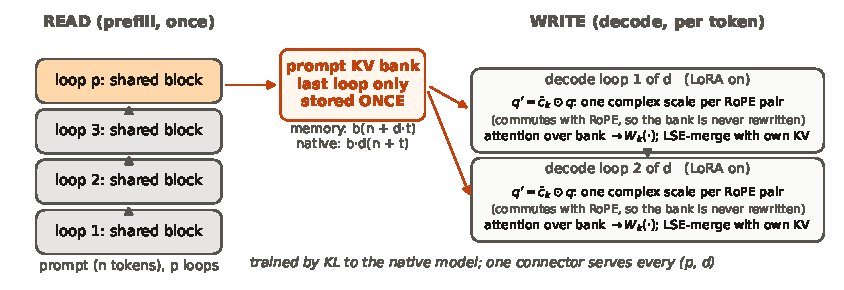
\includegraphics[width=0.95\textwidth]{figs/fig0_method.pdf}
\caption{The depth-split connector. The frozen model reads the prompt with $p$ loops and keeps one prompt KV bank (the
last loop's). Each of the $d$ decode loops reads that bank through its own map: a per-frequency complex key scale,
folded into the query because it commutes with RoPE, and a value map applied after attention; the result is merged by
log-sum-exp with attention over the generated tokens' own KV.}
\label{fig:method}
\end{figure*}

\paragraph{Notation.} ``\rw{p}{d}'' prefills the prompt with $p$ loops and decodes every answer token with $d$ loops;
\nat{d} is the unmodified model.

\paragraph{Prefill.} The frozen model reads the prompt with $p$ loops and keeps only the last loop's prompt keys and
values (one bank, RoPE applied).

\paragraph{Decode.} The same frozen model, with rank-16 LoRA~\citep{lora} on the attention projections, runs $d$ loops
per token. Decode loop $k$ reads the prompt bank through a map indexed by $(k,\text{layer},\text{KV head})$ (Figure~\ref{fig:method}):
\begin{itemize}
\setlength\itemsep{0.1em}
\item \emph{Key map}: one complex scale $c_j$ per rotary frequency pair $j$. Writing a rotated key pair as a complex
number $\tilde k_j = e^{i m\theta_j} k_j$, scaling commutes with the rotation, $c_j\tilde k_j = e^{im\theta_j}(c_jk_j)$,
and $\mathrm{Re}\langle q_j, c_j\tilde k_j\rangle = \mathrm{Re}\langle \bar c_j q_j, \tilde k_j\rangle$. The map is therefore
applied to the query ($q' = \bar c \odot q$) and the stored cache is never rewritten.
\item \emph{Value map}: a full $D\times D$ linear map $W_k$ per head. Because attention is linear in the values,
$\sum_i a_i W_k v_i = W_k\sum_i a_i v_i$: the map is applied once to the attention output over the prompt.
\item Prompt and generated tokens share one softmax: the prompt part and the generated part are computed as two
attention calls and merged by their log-sum-exp; only generated tokens keep per-loop KV (their number $t \ll n$).
\end{itemize}
The prompt KV is thus one loop's worth for every $d$ (``single bank''): total KV is $b(n+d\,t)$ for batch $b$, prompt
length $n$ and $t$ generated tokens, versus $b\,d(n+t)$ for the native model. The single-bank form is algebraically
equal to materialising a transformed prompt cache per loop; in BF16, greedy decisions matched on all 512 checked steps.

\paragraph{Training.} We minimise $\mathrm{KL}(\text{teacher}\,\|\,\text{student})$ over all answer positions, with the
native 4/4 model as teacher, on 48M answer tokens of a mixture of reasoning traces, instruction data, long-context data
and web text. One $(p,d)$ cell is sampled per micro-batch, so a single set of parameters (63M, 2.4\% of the model)
serves all 16 cells. The base model stays frozen; LoRA is merged at serving time.

\section{Setup}
\label{sec:setup}

\paragraph{Models.} Ouro-2.6B (main, 4 loops), Ouro-1.4B (scale), Nanbeige4.2-3B (second family, 2 loops) and
Ouro-2.6B-Thinking and Ouro-1.4B-Thinking (reasoning models, zero-shot with the chat template)~\citep{ouro}, and
SenseNova-Loop-9B-Preview (third family: a hybrid of Gated-DeltaNet and full-attention layers whose middle block is
visited twice; \S\ref{sec:sensenova}).

\paragraph{Benchmarks.} Full or large sets: GSM8K~\citep{gsm8k} (1,319; 3-shot CoT for base models, zero-shot for
thinking models), MMLU~\citep{mmlu} (14,042; 5-shot), RULER~\citep{ruler} 4K/8K/16K (520 each), HELMET~\citep{helmet}
(1,108), BBH~\citep{bbh} (3-shot CoT, 1,620), MMLU-Pro~\citep{mmlupro} (5-shot CoT, 980), ARC-Challenge~\citep{arc}
(25-shot, 1,172), MATH-500~\citep{math} and HumanEval~\citep{humaneval}. We use lm-evaluation-harness prompts and
math-verify scoring; Ouro's native numbers reproduce. All comparisons are paired (same items) with 95\% bootstrap
intervals.

\paragraph{Comparisons.} Three numbers isolate the effects: \nat{d}; the connector at \rw{d}{d}, which carries the same
adaptation; and \rw{p}{d} with $p > d$. Only the last two isolate reading depth; against the native model, gains include
adaptation.

\section{Results}

\subsection{Reading buys understanding, writing buys derivation}

Figure~\ref{fig:grid} shows the full grid for Ouro-2.6B. MMLU rises from 52--53 at read~1 to 70--75 at read~3--4,
independent of writing depth; RULER-16K rises from 53--56 to 62--74. GSM8K barely moves along a row at write~1 (46--55)
and rises with writing depth (to 78--88 at write~3--4). Untrained, the frozen model reading deep KV still gains MMLU, but
GSM8K and RULER collapse at write~1--2 (\rw{4}{1}: GSM8K 13.0, RULER-16K 7.6): the connector is what makes the
combination usable.

Table~\ref{tab:equal} isolates reading depth within the connector. At one writing loop, reading 4 loops instead of 1
adds 15.2 MMLU, 8.0 GSM8K and 8.6 RULER-16K points. The gain shrinks as writing deepens: a deep writer reads its own
deep prompt representation anyway. On RULER, the read-deep gain grows with prompt length---negative at 4K, positive at
16K---and most of it comes from the second prefill loop (RULER-16K at write~1: 54.3 / 61.6 / 61.3 / 62.8 for read 1--4).

\begin{table}[t]
\centering\small
\setlength\tabcolsep{3pt}
\begin{tabular}{@{}lccc@{}}
\toprule
write $d$ & MMLU & GSM8K & RULER-16K \\
\midrule
1 & $+15.2$\ci{14.3}{16.1} & $+8.0$\ci{5.4}{10.5} & $+8.6$\ci{4.2}{12.9} \\
2 & $+6.0$\ci{5.3}{6.7} & $-1.7$\ci{-3.5}{0.1} & $+5.3$\ci{1.2}{9.3} \\
3 & $+0.6$\ci{0.2}{1.1} & $-0.8$\ci{-2.4}{0.8} & $-0.4$\ci{-3.0}{2.2} \\
\bottomrule
\end{tabular}
\caption{Reading depth at equal writing depth (Ouro-2.6B, one connector): \rw{4}{d} minus \rw{d}{d}, full sets. RULER
4K at write~1: $-3.8$\ci{-7.8}{0.3}.}
\label{tab:equal}
\end{table}

Table~\ref{tab:bench} extends the comparison against the native model to five more benchmarks. At one writing loop,
reading deep adds 15--23 points on BBH, MMLU-Pro, ARC-C and HELMET; at write~2, HELMET reaches the native 4/4 level
(53.0 vs.\ 54.8). MATH-500 is the exception (\S\ref{sec:limits}).

\begin{table}[t]
\centering\small
\setlength\tabcolsep{2.5pt}
\begin{tabular}{@{}lccccc@{}}
\toprule
$d$ & BBH & MMLU-Pro & ARC-C & HELMET & MATH \\
\midrule
1 & $+20.9$ & $+21.4$ & $+14.8$ & $+23.3$ & $-6.0$ \\
2 & $+4.6$ & $+7.8$ & $+2.9$ & $+28.0$ & $-2.6$ \\
3 & $-1.1$ & -- & $+0.3$ & $+5.0$ & $-2.2$ \\
\bottomrule
\end{tabular}
\caption{\rw{4}{d} minus \nat{d}, Ouro-2.6B. Write~1 intervals: BBH \ci{18.0}{23.9}, MMLU-Pro \ci{18.2}{24.7},
ARC-C \ci{12.1}{17.3}, HELMET \ci{20.3}{26.5}, MATH \ci{-10.2}{-2.2}.}
\label{tab:bench}
\end{table}

\paragraph{Generalisation.} The read-depth effect holds across scale, family and training stage (Table~\ref{tab:gen}).
On Nanbeige4.2-3B (two loops) the comparison uses separately trained per-cell connectors, so reading depth and connector
weights change together; a single universal connector for Nanbeige suffers interference between read depths
(\S\ref{sec:limits}).

\begin{table}[t]
\centering\small
\setlength\tabcolsep{3pt}
\begin{tabular}{@{}p{0.27\columnwidth}p{0.66\columnwidth}@{}}
\toprule
model & \rw{4}{1} $-$ \nat{1} (unless noted) \\
\midrule
Ouro-1.4B & RULER-16K $+14.3$, MMLU $+22.4$, GSM8K $+14.9$, ARC-C $+17.2$; BBH $-11.7$ (collapse, \S\ref{sec:limits}) \\
Nanbeige4.2-3B & \rw{2}{1} $-$ \rw{1}{1}: RULER 4K/8K/16K $+11.8/+11.7/+11.0$, MMLU $+12.2$, GSM8K $+5.2$, ARC-C $+11.6$ \\
Ouro-2.6B-Thinking & GSM8K $+18.0$\ci{15.2}{20.6}, MATH-500 $+13.2$\ci{8.5}{18.2}, HELMET$^\ddagger$ $+25.6$\ci{22.3}{28.9}, MMLU-Pro $+16.2$, ARC-C $+14.3$ \\
Ouro-1.4B-Thinking & GSM8K $+20.1$\ci{17.1}{23.4}, MMLU-Pro $+15.5$\ci{10.0}{20.7}; within the connector \rw{4}{1} $-$ \rw{1}{1}: GSM8K $+13.6$\ci{10.4}{16.5}, MMLU-Pro $+17.1$\ci{12.4}{22.1}, HELMET$^\ddagger$ $+11.9$\ci{8.9}{14.6}; BBH collapses (\S\ref{sec:limits}) \\
\bottomrule
\end{tabular}
\caption{Same comparison across models (full sets except: BBH 60 per subtask, HELMET 1,108 rows; Nanbeige RULER-16K 385 paired rows; Thinking MMLU-Pro 420 (both sizes),
MATH-500 400). $^\ddagger$Thinking models on raw HELMET prompts are decoded so that an answer cannot be empty
(\S\ref{sec:limits}). All positive entries are significant.}
\label{tab:gen}
\end{table}

\subsection{Shallow writers run out of budget; deep reading helps them finish}
\label{sec:wander}

A reasoning model written with one loop wanders. On Ouro-2.6B-Thinking, \nat{1} hits the 4,096-token budget on 43.5\%
of GSM8K problems (almost every unfinished answer is a budget hit, not an early stop) and uses 15.7 hesitation markers
(``wait'', ``alternatively'', ``re-read'') per 1,000 tokens (Table~\ref{tab:wanderdec}). Training the connector at
\rw{1}{1} halves the budget hits---an adaptation effect. With the writer fixed, reading 4 loops instead of 1 cuts them
further (19.8\% $\to$ 13.0\%), shortens answers by 20\% and adds 6.6 accuracy points (on Ouro-1.4B-Thinking:
$+13.6$\ci{10.4}{16.5}, answers without \verb|\boxed{}| 37.7\% $\to$ 26.0\%), and the gain grows with problem
difficulty (Figure~\ref{fig:wander}): on problems whose reference solution has five or more steps, \rw{4}{1} gains 10
points over \rw{1}{1}. Hesitation \emph{density} does not fall (12.2 vs.\ 13.8 per 1,000 tokens): the deep-reading writer
does not hesitate less per step, it reaches an answer in fewer steps. At two writing loops the increment is small on
GSM8K (\rw{2}{2} 92.8 vs.\ \rw{4}{2} 93.3; 858 vs.\ 836 tokens), and both track \nat{4}.

\begin{table}[t]
\centering\small
\setlength\tabcolsep{3pt}
\begin{tabular}{@{}lrrrr@{}}
\toprule
config & acc. & budget hit & tokens & marks/1k \\
\midrule
\nat{1} & 59.7 & 43.5\% & 2,286 & 15.7 \\
\rw{1}{1} & 71.1 & 19.8\% & 1,392 & 12.2 \\
\rw{4}{1} & 77.7 & 13.0\% & 1,113 & 13.8 \\
\nat{2} & 92.2 & 6.3\% & 957 & 7.8 \\
\rw{2}{2}$^\dagger$ & 92.8 & 4.4\% & 858 & 5.8 \\
\rw{4}{2} & 93.3 & 3.9\% & 836 & 5.8 \\
\nat{4} & 94.2 & 3.2\% & 816 & 5.2 \\
\bottomrule
\end{tabular}
\caption{Ouro-2.6B-Thinking, GSM8K zero-shot (1,319; $^\dagger$989). Budget hit: answer reached 4,096 tokens.
Marks: ``wait / alternatively / re-read'' per 1,000 generated tokens.}
\label{tab:wanderdec}
\end{table}

\subsection{A third family: SenseNova-Loop-9B, with and without training}
\label{sec:sensenova}

SenseNova-Loop-9B-Preview is a 9B hybrid of Gated-DeltaNet and full-attention layers whose middle 24 of 32 layers are
visited twice. Its one-visit writer collapses (\nat{1}: 2.2\% GSM8K, 96.8\% of answers without a final \verb|\boxed{}| answer, 86 ``wait / re-read /
alternatively'' per answer), which makes it a clean test (Table~\ref{tab:sn}).

\paragraph{Without any training.} Handing the same one-visit writer the two-visit prefill state---full-attention KV and
the Gated-DeltaNet convolution and recurrent states of the last visit, no parameter changed---cuts unanswered GSM8K
problems (no \verb|\boxed{}|) to 43.7\% ($-53.1$\ci{-55.7}{-50.3}), raises RULER-4K from 21.6 to 83.5 and MMLU-Pro from 18.9 to 55.1
($+36.2$\ci{32.8}{39.7}). The writer, its depth and its weights are identical; only what it reads differs. The
intervention transfers the whole state---attention KV and Gated-DeltaNet state---so it does not separate the two; RULER
uses a non-thinking prefill for every configuration, because the model otherwise spends the 64-token budget thinking.

\paragraph{With a connector.} An 11M-parameter LoRA connector (20M KL tokens; Appendix~\ref{app:training}) trained for a
single one-visit decoder that reads either a one- or a two-visit prompt state removes the collapse, an adaptation effect: GSM8K reaches the
\nat{2} level whichever depth it reads, and end to end \rw{1}{1} takes $0.59\times$\ci{0.52}{0.68} the time of \nat{2}
and \rw{2}{1} $0.64\times$\ci{0.50}{0.83} (64 problems, batch 1; 74 and 80 vs.\ 131 ms per token, close to 32 vs.\ 56
layer executions). Reading depth then shows where
the thesis predicts: with the same decoder, reading two visits beats reading one on long-context HELMET by
$6.7$\ci{5.8}{7.7} points, on MMLU-Pro by $5.5$\ci{3.0}{8.1} and on 3-shot BBH by $7.0$\ci{5.9}{8.0} (BBH: all
6,511 problems; \nat{2} 57.6, \nat{1} 2.6),
while on RULER it costs 3.7 points at 4K and is neutral at 16K ($+1.2$\ci{-1.7}{4.0}), as on Ouro at short contexts.

\begin{table}[t]
\centering\small
\setlength\tabcolsep{2.2pt}
\begin{tabular}{@{}lrrrrrrr@{}}
\toprule
config & GSM8K & unfin. & R-4K & R-8K & R-16K & HELMET & MMLU-Pro \\
\midrule
\nat{1} & 2.2 & 96.8 & 21.6 & 16.5 & 14.0 & 12.3 & 18.9 \\
\rw{2}{1}, no training & 10.9 & 43.7 & 83.5 & 80.8 & 80.6 & 69.5 & 55.1 \\
\rw{1}{1} + connector & 95.6 & -- & 85.8 & 83.3 & 81.5 & 60.9 & 60.3 \\
\rw{2}{1} + connector & 95.2 & -- & 82.1 & 81.4 & 82.7 & 67.6 & 65.8 \\
\nat{2} & 95.8 & 0.3 & 86.9 & 85.8 & 86.1 & 71.8 & 68.2 \\
\bottomrule
\end{tabular}
\caption{SenseNova-Loop-9B-Preview. GSM8K zero-shot chat (1,319); RULER with a non-thinking prefill (520 per length);
HELMET (6,646); MMLU-Pro 5-shot CoT (980).}
\label{tab:sn}
\end{table}

\begin{figure*}[t]
\centering
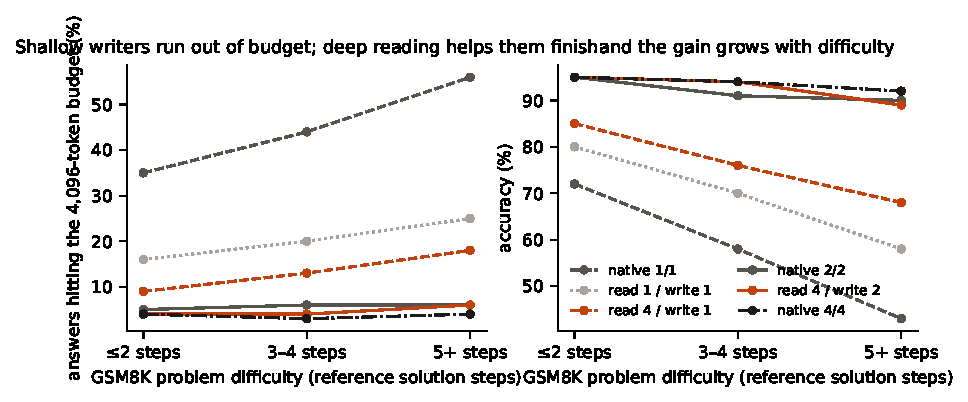
\includegraphics[width=0.85\textwidth]{figs/fig3_wandering.pdf}
\caption{Ouro-2.6B-Thinking on all 1,319 GSM8K problems, bucketed by reference-solution steps.}
\label{fig:wander}
\end{figure*}

\begin{table}[t]
\centering\small
\setlength\tabcolsep{2.5pt}
\begin{tabular}{@{}lrrrr@{}}
\toprule
config & acc. & tok./ans. & ms/tok. & s/ans. \\
\midrule
\nat{1} & 62.5 & 2,500 & 34.6 & 86.5 \\
\rw{4}{1} & 73.4 & 1,310 & 41.9 & 55.1 \\
\nat{2} & 95.3 & 1,044 & 66.9 & 70.0 \\
\rw{2}{2} & 96.9 & 755 & 82.7 & 62.6 \\
\rw{4}{2} & 96.9 & 741 & 84.9 & 63.1 \\
\nat{4} & 93.8 & 879 & 129.6 & 114.2 \\
\bottomrule
\end{tabular}
\caption{End to end per answer (Ouro-2.6B-Thinking, GSM8K, 64 problems, batch 1, one B300, prefill included, real
greedy answers). On all 1,319 problems: \rw{4}{2} 93.3, \nat{4} 94.2, paired $-1.0$\ci{-2.0}{0.1}.}
\label{tab:e2e}
\end{table}

\paragraph{End to end.} Shallow writing through the connector pays end to end (Table~\ref{tab:e2e}, Figure~\ref{fig:frontier}). \rw{4}{2} answers in $0.55\times$ the time of \nat{4} and $0.90\times$ that of \nat{2}.
We state the cost plainly: at batch~1, single-bank decoding is $1.27\times$ slower per token than \nat{2} (two attention
calls and a merge per layer); the answer arrives sooner because it is 29\% shorter. On all 1,319 problems \rw{4}{2} is
within one point of \nat{4} (93.3 vs.\ 94.2) and above \nat{2} (92.2; $+1.1$\ci{-0.2}{2.4}). The saving over \nat{4}
comes from writing two loops through the connector, not from reading deeper: \rw{2}{2} is as fast and as accurate on the
same problems (\rw{4}{2} takes $1.01\times$\ci{0.91}{1.11} the time of \rw{2}{2}; \rw{2}{2} takes $0.55\times$\ci{0.46}{0.64}
that of \nat{4}). The same holds on MATH-500
(40 problems, 8,192-token budget): \rw{4}{2} matches \nat{4} (85.0 vs.\ 82.5\%) at $0.63\times$\ci{0.53}{0.77} its time,
but is $1.22\times$\ci{1.04}{1.44} slower than \nat{2} at equal accuracy, because its MATH solutions are not shorter. At
write~2, reading deeper pays on long-context reading and knowledge instead (\rw{4}{2} minus \rw{2}{2}:
HELMET $+15.8$\ci{13.1}{18.5}, ARC-C $+2.3$, BBH $+2.2$; on HELMET \rw{4}{2} is $26.0$\ci{22.9}{29.1} points above \nat{2} and $4.3$\ci{2.5}{6.2} above \nat{4}).

\begin{figure}[t]
\centering
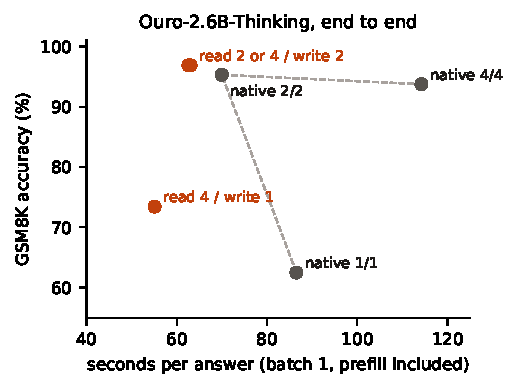
\includegraphics[width=0.9\columnwidth]{figs/fig2_frontier.pdf}
\caption{Accuracy vs.\ time per answer (Table~\ref{tab:e2e}). Dashed: native models. Reading 2 or 4 loops before writing 2 gives the same point.}
\label{fig:frontier}
\end{figure}

\subsection{Serving one prompt bank}

With a static prompt cache and the same fused attention on both sides (FlashAttention-2~\citep{flashattn2} calls merged
by log-sum-exp), the best decode throughput over batch sizes at 8K context is $0.97\times$, $1.19\times$, $1.36\times$
and $1.62\times$ that of the native model at writing depths 1--4, because the single bank admits larger batches as $d$
grows (max batch 64 vs.\ 80/40/24/20). Against the quality reference \nat{4}, \rw{4}{1} decodes $6.5\times$ faster
(813 vs.\ 125 tokens/s). These ratios are against the fastest of three native implementations we measured: static per-loop banks with the same
two-call flash attention as ours (834 / 342 / 125 tokens/s at $d=1/2/4$), ahead of the standard dynamic cache
(500 / 245 / 105) and of a preallocated contiguous cache with one attention call per layer (267 / 130 / 57, slower because
the model's attention mask keeps it off the flash kernel); all variants produce identical greedy tokens. All serving numbers are decode-only; end-to-end cost is in Table~\ref{tab:e2e}.

\subsection{Storing the answer once, too}
\label{sec:selflive}

The single bank stores the prompt once, but generated tokens still keep one KV bank per writing loop: $b(n+d\,t)$.
Sharing one answer bank across loops is what BeNice!~\citep{benice} trains for; its training lets each token read its own
last-loop KV on the diagonal, which does not exist yet at inference. We train the connector directly in the inference-time
view instead (\emph{self-live}\footnote{Self-live was developed by the author in separate work on shared KV caches for
looped models; here it is applied to the connector's answer tokens.}): each writing loop reads the prompt, a single answer history written by the last loop,
strictly before the current token, and on the diagonal only the KV computed live in the current loop; the history comes
from a no-grad pass of the same model (Appendix~\ref{app:training}). The answer is then stored once. Against the same
connector with per-loop answer banks, no difference is significant at two and three writing loops on GSM8K
(\rw{4}{2}: $+0.3$\ci{-1.5}{2.2}; \rw{4}{3}: $+0.5$\ci{-0.9}{2.1}; \rw{3}{3}: $-0.8$\ci{-2.4}{0.8}), MMLU
($-0.1$\ci{-0.4}{0.2}) or RULER-4K (four cells); the cost appears as more loops share one history: MATH at three writing
loops $-3.4$\ci{-6.8}{-0.2}, GSM8K at four $-2.6$\ci{-4.1}{-1.0} (and $-4.8$ against \nat{4}). Our evaluation of this arm materialises the per-loop mapped prompt
banks; serving with one prompt bank and one answer bank (total KV $b(n+t)$, that of a one-loop model) gives the same
greedy tokens (512/512 checked steps). Where answers are long (1K-token prompts, 2,048 generated tokens), it raises the
largest batch that fits from 32 (\nat{4}) and 64 (one prompt bank, per-loop answer banks) to 192, and decode throughput
at four writing loops to $2.17\times$ \nat{4} (476 vs.\ 219 tokens/s; $1.30\times$ \nat{2} at two loops, where
accuracy is unchanged; at four loops the throughput comes with the GSM8K cost above).

\subsection{What each loop stores}
\label{sec:probe}

Why does deep KV help knowledge and long-context reading but hurt verbatim recall (\S\ref{sec:limits})? We fit linear
probes to the frozen native model's per-loop \emph{value} cache---what attention reads back from the prompt---at the
same layer and with the same weights, varying only the loop (Figure~\ref{fig:probe}). Averaged over probed layers, the
previous token is less linearly decodable from loops 2--4 than from loop 1 (Ouro-2.6B: 57.7\% $\to$ 45.5\%, lower in 12 of 13
probed layers), and the next token more (26.0\% $\to$ 36.1\%, higher in all 13); Ouro-1.4B and Ouro-2.6B-Thinking agree. In the hybrid
SenseNova-Loop-9B (six full-attention layers in the looped block, visit 1 vs.\ 2) the next-token gain replicates in every
layer ($24.1\% \to 29.1\%$), but the previous token is about as decodable at both visits on average (56.8\% vs.\
56.5\%; $-7.0$ at the first of these layers, $+2$ to $+3$ at the last); only attention values are probed, not the
Gated-DeltaNet state. The literal loss happens at the second loop, as does the
behavioural one: for few-shot MATH, reading 2 or 3 loops is no better than 4; and the behavioural loss disappears, and
turns into a gain ($+7.0$), when the exemplars that must be imitated are removed.

These are decodability results, not proof of information loss or causal use~\citep{presenthard}, and next-token
prediction is only a proxy for meaning. Not every layer follows the mean (at layer~0, the previous token becomes more
decodable after loop 1). The trend is the across-loop analogue of the across-layer one of \citet{voita2019bottom};
per-loop readouts of Ouro's residual stream show a related latent-prediction trend~\citep{monitorloop}, and per-loop
probes go back to \citet{loopedicl}. What is specific here is the matched-layer comparison of the stored cache: in a
looped model, choosing which loop's KV to keep is choosing what to remember.

\begin{figure*}[t]
\centering
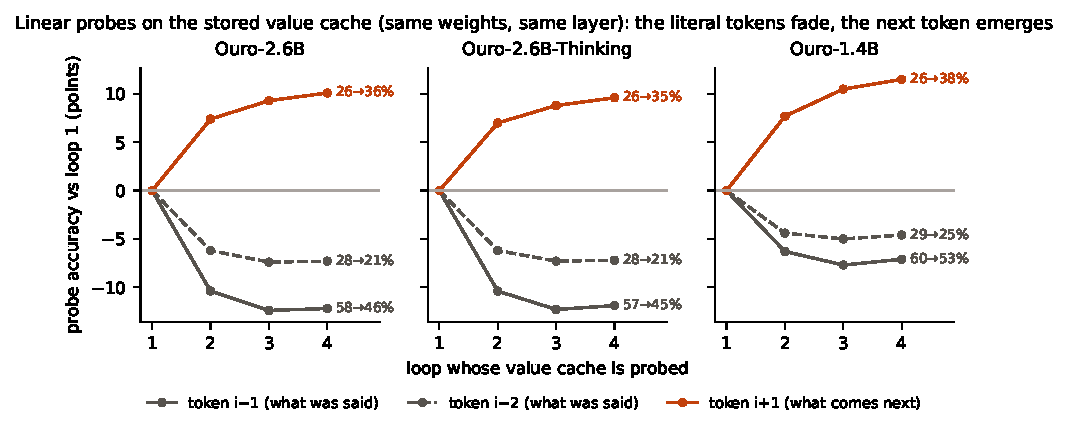
\includegraphics[width=0.85\textwidth]{figs/fig4_probe.pdf}
\caption{Linear probes on the per-loop value cache of three frozen models, change from loop 1 (mean over 13 / 13 / 9 layers; 384 FineWeb windows of 1,024 tokens, 20\% held out; 2,048 most frequent training tokens).}
\label{fig:probe}
\end{figure*}

\subsection{Ablations}
\label{sec:ablations}

\paragraph{Plain sharing.} A trained terminal-KV sharing baseline in the style of BeNice!~\citep{benice} (the decoder
reads the prefill's last-loop KV with LoRA but no map) loses $17.5$\ci{-20.2}{-14.8} GSM8K points at write~1 against our
connector, and ties it at write~2 ($-0.1$\ci{-2.0}{1.7}). The map is what makes one-loop writing over deep KV work; from
two writing loops on, plain sharing suffices.

\paragraph{Giving the writer the first loop back.} If short-context recall suffers because deep KV keeps less of what
was said, handing the writer the \emph{first} prefill loop's KV should help. A gated attention branch over the first
loop's prompt KV (initialised closed; trained like the connector) raises RULER-4K at \rw{4}{1} by
$2.3$\ci{1.0}{3.6}, recovering about 60\% of the read-deep loss, and changes nothing else (GSM8K $+0.7$\ci{-0.8}{2.2},
MMLU $+0.0$; other cells within $\pm0.6$ on RULER-4K, two of them on 406 and 334 of 520 rows). It does not help at two writing loops, and it does not remove the
4-shot MATH loss (22.2 vs.\ 32.2, as without the branch). We report this without a causal reading: the branch adds a
bank and parameters as well as shallow information.

\paragraph{A second training seed.} Retraining the universal connector with another seed (initialisation and cell
sampling) reproduces every read-depth effect on full sets, e.g.\ at one writing loop MMLU $+15.2$ and RULER-16K $+8.6$
under both seeds (Appendix~\ref{app:seed}).

\paragraph{One bank vs.\ one per loop.} Storing a separate mapped bank per decode loop is equal cell by cell (RULER
intervals include zero), so the single bank costs nothing.

\section{Related Work}

\paragraph{Looped and elastic depth.} Accordion~\citep{accordion} and Elastic Latent Recurrence~\citep{elr} serve several
depth budgets from one model trained for it; ELR reports that keeping only the last loop's KV retains most of the gain,
the from-scratch counterpart of our single bank. The Parallel Loop Transformer~\citep{plt}, LoopCoder-v2~\citep{loopcoder2}
and shared-memory looped transformers~\citep{sharedmem} instead share the \emph{first} loop's KV. None decouple prefill
from decode depth; their opposite choices bracket our finding that deep KV serves knowledge and shallow KV serves recall.

\paragraph{Unequal prefill and decode compute.} CDB~\citep{cdb}, OverFill~\citep{overfill}, Position-Aware Depth Decay
Decoding~\citep{padd} and Fixed Points Part~II~\citep{fixedpoints2} use deeper prefill than decode; POP~\citep{pop} and
SPEED~\citep{speed} use the reverse; Decode-Branch Transformers~\citep{decodebranch}, PHD~\citep{phd} and
State-Prediction Separation~\citep{sps} add decode-side computation. We contribute a measurement of what each side buys
and a connector that makes the full grid usable on existing looped checkpoints.

\paragraph{Cross-loop and cross-model KV.} Looped Latent Attention~\citep{lla} compresses KV across loops,
BeNice!~\citep{benice} and LSTM-style looped transformers~\citep{lstmloop} share it; Cache-to-Cache~\citep{c2c},
HeteroFold~\citep{heterofold}, Swarm Telepathy~\citep{swat} and CacheLink~\citep{cachelink} transfer KV between models,
and BellowsKV~\citep{bellows} shares a latent across layers. Like CacheLink, we train maps through the receiver's output
distribution, never on KV reconstruction; within one model, tokens, layers and positions align, so a RoPE-commuting scale
and a value map suffice and are exact to serve.

\section{Conclusion}

Depth in a looped model is not one budget but two. Reading depth buys understanding and is paid once; writing depth buys
derivation and is paid per token. A small connector makes the two separable on existing checkpoints, a RoPE-commuting
map lets one prompt cache serve every writing depth, and reading deeper lets a shallow writer reason with less wandering
and in less time.

\section*{Limitations}
\label{sec:limits}

\paragraph{Short-context recall and few-shot mathematics prefer shallow KV.} Within the connector at one writing loop,
reading 4 loops instead of 1 lowers RULER-4K ($-3.8$\ci{-7.8}{0.3}) and 4-shot MATH-500 on the base model
($-9.8$\ci{-13.8}{-5.8}; $-11.2$\ci{-15.6}{-7.0} with the same full-answer scoring as below); RULER at 16K moves the other
way. On MATH the sign depends on prompting: with the same connector and problems but no exemplars, reading deep
\emph{helps} ($+7.0$\ci{3.2}{11.0}; 40.8 vs.\ 33.8), and the
reversal replicates at two writing loops (read 4 vs.\ 2: $+7.0$\ci{3.0}{10.8}) and on Ouro-1.4B ($-4.0$\ci{-8.0}{0.0}
with exemplars, $+4.8$\ci{1.2}{8.2} without). Removing exemplars also changes length and format, so we read this as a prompting interaction consistent with,
not proof of, deep KV keeping less of what was said (\S\ref{sec:probe}). Reading fewer loops avoids the loss when
exemplars are given.

\paragraph{Deep writing over one deep bank loses retrieval.} At three or more writing loops, the single-bank connector
trails \nat{d} on RULER (write~3: $-10.4/-9.5/-5.3$ at 4K/8K/16K), because the native model reads a separate prompt bank
per loop.

\paragraph{Deeper prefill costs time to first token.} Reading 4 loops costs a 4-loop prefill: in an interim batch-1
measurement on RULER-16K (64-token answers), a \rw{4}{1} request took about $1.6\times$ \nat{1} and half of \nat{4}.
Deep reading pays for itself only when answers are long or quality requires it.

\paragraph{Transfer is not free.} On Nanbeige4.2-3B one universal connector suffers interference between read depths;
per-depth adapters fix RULER and MMLU, and doubling the data halves the remaining GSM8K gap.

\paragraph{Collapse at the extreme cell.} Both 1.4B checkpoints degenerate at \rw{4}{1} on 3-shot CoT BBH (Ouro-1.4B:
empty or echoed answers; Ouro-1.4B-Thinking: 28\% empty and $-20.5$ points against \rw{1}{1}); read 1--2, and reading 4
loops at two writing loops ($+8.8$\ci{6.2}{11.5} over \rw{2}{2}), do not.

\paragraph{Empty answers on raw prompts.} Thinking checkpoints given raw (non-chat) HELMET prompts often stop at once
(a newline, then end of sequence): 42.7\% of \nat{2} answers on Ouro-2.6B-Thinking, at most 1.1\% for read-4 connectors.
For thinking models we therefore mask the stop tokens until an answer has a non-whitespace token, for every configuration.
This does not rescue \nat{2} (34.1 vs.\ 31.4): its empty answers hid no correct ones. Base models are unaffected
($\le$2.7\% empty).

\paragraph{Wandering measures.} ``Unfinished'' means the answer hit the generation budget; hesitation markers are
lexical. Neither measures reasoning quality directly.

\paragraph{Scope.} Six looped checkpoints from 1.4B to 9B parameters (the full $4\times4$ grid only on Ouro-2.6B),
greedy decoding, English benchmarks; end-to-end latency at batch~1 on 64 problems and one GPU type. Gains against
native models include adaptation; reading-depth effects are isolated within the connector, or without training
(SenseNova).

\bibliography{references}

\appendix

\section{Training Details}
\label{app:training}

\paragraph{Connector.} Rank-16 LoRA ($\alpha=16$, no dropout) on the query, key, value and output projections, active
only in decode; per (decode loop, layer, KV head) a complex scale for each rotary frequency pair on keys and a full
$D\times D$ value map, both initialised to the identity. Trainable parameters: 63,307,776 for Ouro-2.6B (2.4\%). The
backbone is frozen.

\paragraph{Objective.} $\mathrm{KL}(\text{teacher}\,\|\,\text{student})$ summed over answer positions and normalised by
the number of KL tokens in the global batch; the teacher is the native 4/4 model with the same weights. One cell $(p,d)$
is sampled per micro-batch from all 16 pairs.

\paragraph{Data.} 48M KL tokens: OpenThoughts reasoning traces 45\%, Tulu SFT responses 40\%, LongAlpaca long-context
answers 5\% and FineWeb-Edu windows 10\% (fractions of KL tokens); prompts up to 7,680 tokens, answers up to 1,024. Base
models see a plain ``User: \ldots\ Assistant:'' format; thinking models see the same samples in their chat template. No
benchmark data enters training.

\paragraph{Optimisation.} AdamW ($\beta=(0.9,0.95)$, no weight decay), peak learning rate $10^{-4}$ with 2\% linear warm-up
and cosine decay to $10^{-5}$, gradient clipping at 1.0, global batch 24 sequences on 4 GPUs, bfloat16 backbone.

\paragraph{SenseNova-Loop-9B.} Rank-16 LoRA on the attention projections of the looped layers (full attention: q/k/v/o;
Gated-DeltaNet: input and output projections), active only in decode; no maps. The one-visit decoder reads the prefill
state of the last of $p\in\{1,2\}$ visits (sampled 50/50), so the same decoder serves read~1 and read~2. Teacher: native
2/2. Data: the same mixture re-rendered in the SenseNova chat template (60,000 samples), 20M KL tokens, peak learning rate
$2\times10^{-4}$.

\paragraph{Self-live answer bank.} Generated tokens keep one KV bank per layer shared by all writing loops; at
inference the last writing loop commits each token to it. Training uses the same KL objective as the connector, computed
through the inference-time view in two passes: a no-grad pass in which each loop reads its own causal answer KV records
the last loop's answer KV; a second pass reads, at every loop, the prompt bank, that recorded history strictly before the
current position, and the current token's live KV on the diagonal. Prompt side, data and budget as for the connector.

\section{Evaluation Details}
\label{app:eval}

All tasks run through lm-evaluation-harness with greedy decoding and our runner. Base models: GSM8K 3-shot CoT (1,319),
MMLU 5-shot (14,042), BBH 3-shot CoT (60 per subtask, 1,620), MMLU-Pro 5-shot CoT (70 per subject, 980), ARC-Challenge
25-shot (1,172), MATH-500 4-shot Minerva, HumanEval. Long context: RULER 4K/8K/16K (520 rows each, 13 tasks $\times$ 40)
and HELMET (1,108). Thinking models: zero-shot with the chat template, answers in \verb|\boxed{}| scored by math-verify,
budget 4,096 tokens (GSM8K) and 8,192 (MATH-500). MATH-500 is scored with math-verify throughout; Minerva's strict
``Final Answer'' match would reverse the 4-shot read-depth comparison on Ouro-2.6B (19.6 vs.\ 9.8) because the read-1
writer drops the required format more often, which is why we do not use it. Intervals are paired bootstrap 95\% over items (2,000 or 5,000 resamples); for
HELMET, resampling clusters equals resampling rows.

\section{Training-Seed Robustness}
\label{app:seed}

\begin{table}[h]
\centering\small
\setlength\tabcolsep{3pt}
\begin{tabular}{@{}llrr@{}}
\toprule
comparison & task & seed 1 & seed 2 \\
\midrule
\multirow{5}{*}{\rw{4}{1} $-$ \rw{1}{1}} & GSM8K & $+8.0$\ci{5.5}{10.3} & $+7.2$\ci{4.5}{9.9} \\
 & MMLU & $+15.2$\ci{14.3}{16.1} & $+15.2$\ci{14.4}{16.2} \\
 & RULER-4K & $-3.8$ & $-3.5$ \\
 & RULER-8K & $+2.5$ & $+2.0$ \\
 & RULER-16K & $+8.6$\ci{4.5}{12.5} & $+8.6$\ci{4.1}{12.6} \\
\midrule
\multirow{2}{*}{\rw{4}{2} $-$ \rw{2}{2}} & GSM8K & $-1.7$\ci{-3.5}{0.2} & $-2.9$\ci{-4.8}{-1.0} \\
 & RULER-4K & $-7.2$ & $-6.8$ \\
\bottomrule
\end{tabular}
\caption{Ouro-2.6B universal connector trained with two seeds; paired differences within each seed on full sets.}
\end{table}

\section{Compute}

The universal Ouro-2.6B connector trains in 6.7 hours on 4 B300 GPUs (48M KL tokens). Evaluations, probes and timing used two 8-GPU B300 nodes;
end-to-end timing uses one otherwise idle GPU per configuration.

\end{document}
